%Autor: Simon Walker
%Version: 1.0
%Datum: 30.04.2020
%Lizenz: CC BY-NC-SA

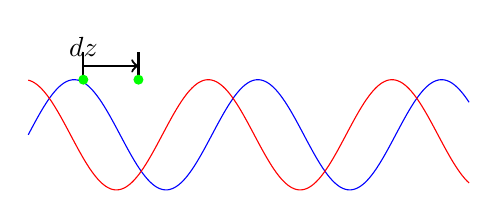
\begin{tikzpicture}[xscale=0.7, yscale=0.7]
	%\HelpCords{0}{-1}{9}{1}
	
	\def\l{8} %Länge der Schwingungen
	\def\o{0.9} %Offset (Positiv bedeutet Rot links von blau)
	\def\f{0.3} %Frequenz der Schwingunen
	
	\tikzmath{
		\p1 = 450/(360*\f); %Peek1
		\p2 = \p1 - \o; %Peek2
		\pl = (\p1+\p2)/2;
	}
	
	\draw[blue] plot[domain=0:\l, samples=200] 
	(\x, {sin(360*\f*\x});
	\draw[red] plot[domain=0+\o:\l+\o, samples=200] 
	(\x-\o, {sin(360*\f*\x)});
	
	%\draw[green, *<-*] (\p2, 1) -- (\p1, 1);
	\draw [thick] (\p1, 1) -- (\p1, 1.5);
	\draw [thick](\p2, 1) -- (\p2, 1.5);
	\draw [->, thick] (\p1, 1.25) -- (\p2, 1.25);
	\node[above] at (\pl, 1.25) {$dz$};
	
	\draw[fill=green, green] (\p1, 1) circle [radius=0.08];
	\draw[fill=green, green] (\p2, 1) circle [radius=0.08];
	
\end{tikzpicture}
